\subsection{Boundary conditions}
\label{subsubsec:boundary_conditions}

We now need to set the boundary conditions for the simulations.

The boundary conditions types used for the simulations are reported in Table \ref{tab:boundary_conditions}.

\begin{table}[H]
    \centering
    \begin{tabular}{|c|c|}
        \hline
        \textbf{Boundary} & \textbf{Condition type} \\
        \hline
        Inlet             & Velocity Inlet          \\
        Outlet            & Pressure Outlet         \\
        Rocket Surface    & Wall                    \\
        Domain Surface    & Wall                    \\
        \hline
    \end{tabular}
    \caption{Boundary conditions type used for the CFD simulations.}
    \label{tab:boundary_conditions}
\end{table}


\paragraph{Velocity inlet}

Since our target here is to obtain a drag coefficient that is representative of the average flight conditions, we decided to reduce the speed to $85\%$ of the maximum one.
Based on the data collected from the performed flight, we know that the rocket reached a maximum speed of $\approx 127m/s$.
By computing $85\%$ of this value, we get a speed of $\approx 110m/s$.

This is a strong approximation, given that the drag coefficient $C_d$ is also function of the speed of the flow (see Figure \ref{fig:velocity_inlet}).

\begin{figure}[H]
    \centering
    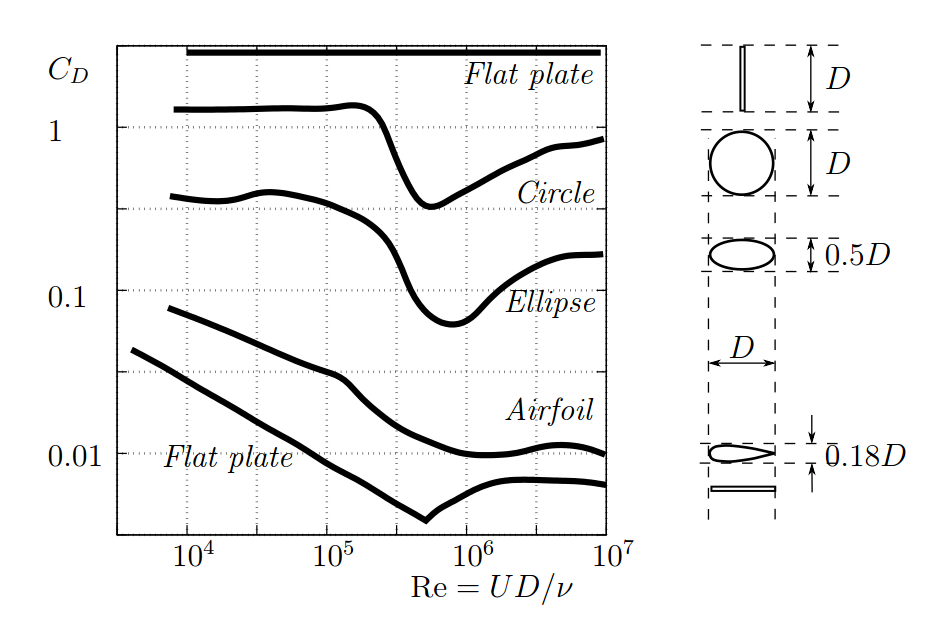
\includegraphics[width=.7\textwidth]{img/Cd_vs_Re.png}
    \caption{Drag coefficient $C_d$ as a function of the Reynolds number $Re$ for different shapes of the object.}
    \label{fig:velocity_inlet}
\end{figure}

From Figure \ref{fig:velocity_inlet} we can see that the drag coefficient $C_d$ changes significantly at low Reynolds numbers and has a drop across the transition from laminar to turbulent regime for non-slender bodies.

From a quick and approximated calculations we can clearly see that the rocket operate in the turbulence region for most of the flight duration, where the rate of change of the drag coefficient is less pronounced.
In particular, considering a set of velocities we can compute the Reynolds number $Re$ as:

\begin{equation}
    Re = \frac{\rho v L}{\mu} = \begin{cases}
        v = 110m/s \rightarrow Re = 4.9 \cdot 10^6 \\
        v = 50m/s \rightarrow Re = 2.2 \cdot 10^6  \\
        v = 10m/s \rightarrow Re = 4.5 \cdot 10^5  \\
    \end{cases}
\end{equation}

Where $\rho$ (density of the fluid) and $\mu$ (dynamic viscosity of the fluid) have been considered constant and equal to $1.225kg/m^3$ and $1.789 \cdot 10^{-5}kg/(m \cdot s)$ respectively.


\paragraph{Pressure outlet}

To set the pressure outlet inside the \texttt{Fluent} solver, we need to specify it as a gauge pressure.

For simplicity (and lack of experience with the software), we set the gauge pressure to $0Pa$.
This is equivalent to say that at the outlet boundary, the pressure is equal to the atmospheric pressure.

However, if we suppose that the atmospheric pressure considered by the software is the standard atmospheric pressure at sea level ($101325Pa$), this might result in a slight approximation of the simulation.

In fact, given that as stated in Table \ref{tab:conditions} the altitude of the starting point of the rocket is $1444m$ (meters above sea level), the atmospheric pressure is lower than the standard atmospheric pressure at sea level.
In particular, if we consider ideal gas law for the air flow, we can compute the atmospheric pressure at a given altitude as:

\begin{align}
    \frac{p}{\rho}                     & = \frac{RT}{M_{mol}}                                                   \\
    \frac{\nabla p}{p} = \nabla \ln(p) & = - \frac{g M_{mol}}{RT} \nabla \tilde{z}                              \\
    p                                  & = p_0 \exp\left(-\frac{g M_{mol} (\tilde{z} - \tilde{z_0})}{RT}\right)
    \label{eq:atmospheric_pressure}
\end{align}

Where $p$ is the pressure, $\rho$ is the density of the fluid, $R$ is the universal gas constant, $T$ is the temperature of the fluid, $M_{mol}$ is the molar mass of the fluid, $g$ is the acceleration due to gravity, $\tilde{z}$ is the altitude, $\tilde{z_0}$ is the altitude at the sea level and $p_0$ is the standard atmospheric pressure at sea level.

Given Equation \ref{eq:atmospheric_pressure}, we can compute the atmospheric pressure at the launch site, which is at an altitude of $1444m$, as:

\begin{equation}
    p_{launch} = 101325 \exp\left(-\frac{9.81 \cdot \frac{28.96}{1000} \cdot 1444}{8.31 \cdot (273.15 + 15)}\right) = 85378Pa
\end{equation}

We can see that at the launch site the atmospheric pressure is almost $16\%$ lower than the standard atmospheric pressure at sea level.

The difference is even more accentuated if we consider the altitude at the apogee of the rocket, which is around $1979m$.
In this case, the atmospheric pressure is:

\begin{equation}
    p_{apogee} = 101325 \exp\left(-\frac{9.81 \cdot \frac{28.96}{1000} \cdot 1979}{8.31 \cdot (273.15 + 15)}\right) = 80101Pa
\end{equation}

In this case, the atmospheric pressure is almost $21\%$ lower than the standard atmospheric pressure at sea level.

Given these considerations, we can imagine that the approximation of the atmospheric pressure at the outlet boundary of the domain might have a slight impact on the results of the simulations, forcing a small extra force from the bottom of the domain, resulting in a slight decrease of the velocity of the flow.
However, we believe that this approximation is not critical for the results of the simulations.

